\section{Implementazione lato front-end}
\label{frontend}

\subsection{HTML}
Si è deciso di usare xHTML 1.0 per garantire il supporto a tutti i tipi di web browser.
La parte di codifica in xHTML 1.0 ha posto le basi della struttura del sito ed è stata completata, nella sua interezza, come prima cosa.
Questa è stata templatizzata il più possibile per garantirne un riutilizzo efficace. Infatti sono stati creati in prima istanza l’header e il footer, così da poterli utilizzare in ogni pagina, e successivamente sono state creati ad hoc i contenuti di tutte le pagine.
Si è deciso di utilizzare HTML 5 solo per l'utilizzo della mappa interattiva Google Maps tramite il tag \textit{iframe}.


Strumento fondamentale per validare la correttezza del codice xHTML 1.0 e HTML 5 è stato il validatore fornito da W3C. Il validatore è stato settato con Document Type xHTML 1.0 Strict.
Da notare il fatto che le funzionalità HTML 5 sono state implementate per ultime, in maniera tale da preservare le funzionalità principali del sito nel caso in cui si utilizzi un browser che non supporta la suddetta versione di HTML. Questa caratteristica permette al nostro sito di “degradare elegantemente”.
\\
\\
Da menzionare il fatto che si è presa la decisione di definire il current link come classe e non come id, per evitare un conflitto con l’id dell’area medica precedentemente definito.

\subsection{CSS}
Fin da subito si è deciso di progettare 3 fogli di stile separati, rispettivamente: 
\begin{enumerate}
\item Stile desktop;
\item Stile mobile;
\item Stile stampa.
\end{enumerate}

\subsubsection{CSS desktop}
\label{frontend:css}
Scelte degne di nota sono state:
\begin{itemize}
\item Il logo, ritenuto molto importante in quanto associato dai clienti con lo studio, è stato inserito all’interno dell’HTML e poi modificato successivamente in CSS;
\item Tutte le immagini sono state adattate alla pagina usando il CSS;
\item Si è deciso di utilizzare una impostazione a due colonne per la maggior parte delle pagine;
\item Abbiamo differenziato l’uso di bold su CSS e strong/em in HTML, permettendo così il giusto funzionamento della lettura attraverso lo screen reader, sia la correttezza grafica del testo;
\item Per far si che con la riduzione della grandezza della pagina, le immagini del footer non occupino troppo spazio, abbiamo usato \textit{@media (max-width: 906px)}.
\end{itemize}

\subsubsection{CSS mobile}
Le modifiche che abbiamo effettuato per l’adattamento alla versione mobile sono state:
\begin{itemize}
\item L’accesso/registrazione utente sono stati condensati in una singola icona, posta in alto a sinistra, la quale, se cliccata, mostra un piccolo menù a tendina che permette di scegliere se accedere o registrarsi;
\item Il menù di navigazione invece è stato implementato tramite un menù ad hamburger, il quale, al click, diventa un menù a tendina che occupa buona parte dello schermo ma senza nascondere completamente il contenuto della pagina;
\item Sono stati pensati 2 differenti punti di rottura:
\begin{enumerate}
\item Il primo a 630px orizzontali sancisce l’effettivo passaggio alla versione mobile;
\item Il secondo a 500px orizzontali prevede l’adattamento del logo e del titolo che vengono ridotti di circa il 50\%. In questo caso, anche il titolo che precedentemente non poteva essere cliccato, diventa cliccabile per sopperire alla poca superficie occupata dal logo rimpicciolito.
\end{enumerate}
\end{itemize}

\begin{center}
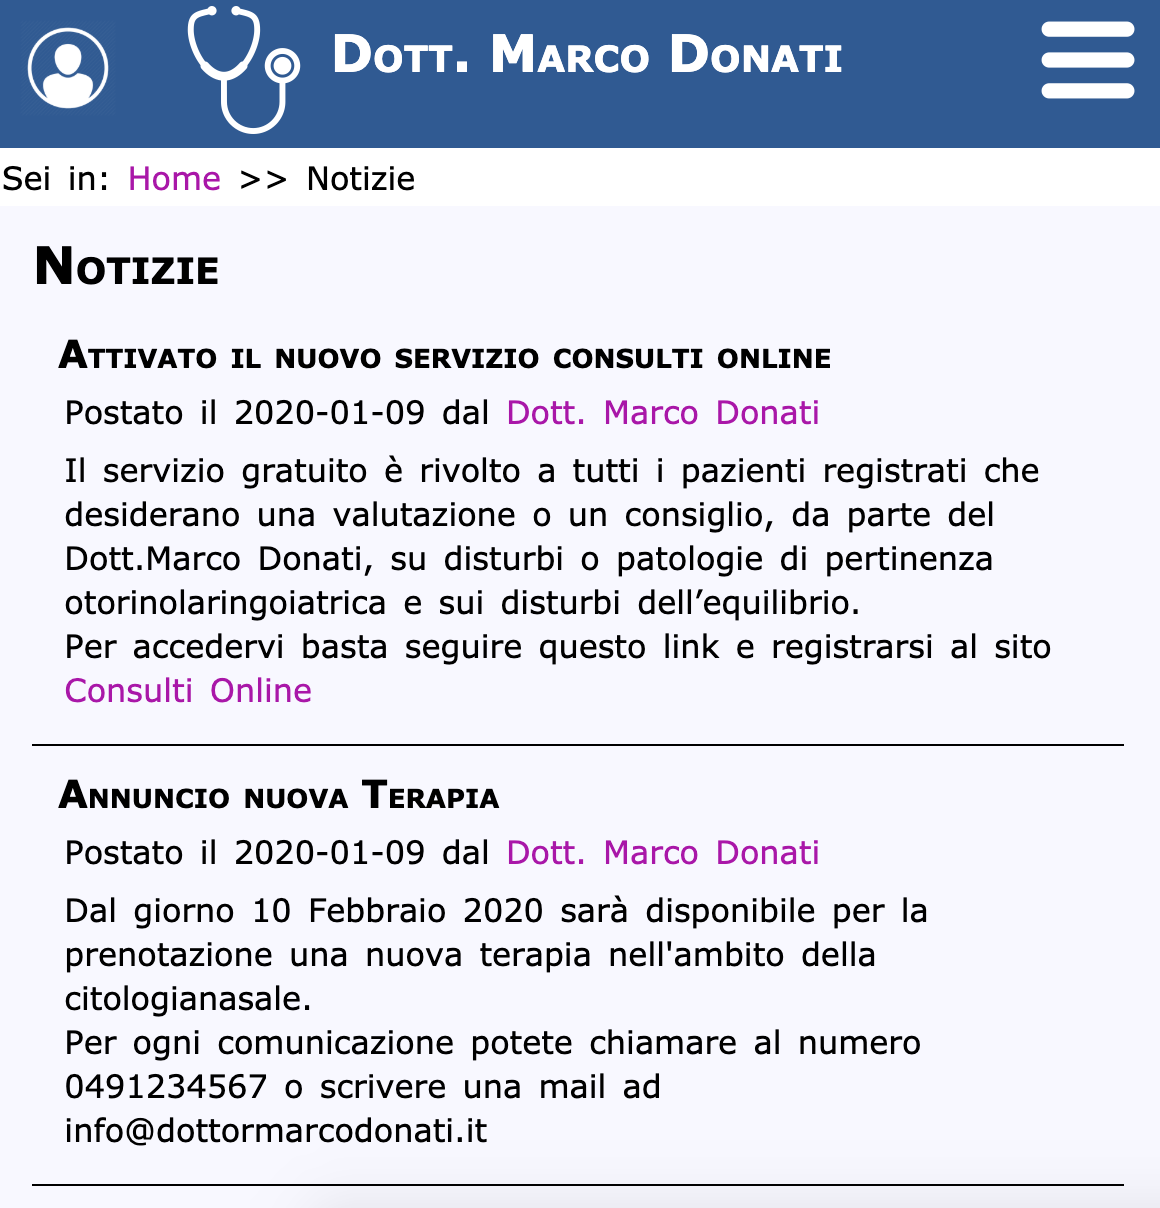
\includegraphics[width=12cm]{../img/mobile}
\end{center}
\captionof{figure}{Esempio di una pagina mobile, in questo caso \textit{Notizie}}

\bigskip

\subsubsection{CSS stampa}
Il CSS  di stampa è stato scritto seguendo tutte le linee guida illustrate a lezione:
\begin{enumerate}
\item I link sono stati colorati in grigio (\#5E5E64) (per garantire una stampa full b/w) e l’indirizzo URL è stato esplicitato;
\item Le breadcrumbs sono state rimosse;
\item Il menù di navigazione è stato rimosso;
\item La mappa di Google Maps è stata rimossa dalla stampa, poiché non è ritenuta utile come immagine statica;
\item La disposizione dei form della pagina Prenota Visita è stata cambiata per esser visualizzata meglio su carta;
\item In alto, accanto alla data, è stata lasciata la stampa dell’id pagina (esempio Consulti \textit{Online-Dott. Marco Donati} per la pagina \textit{consultionline.html}) per dare più contesto;
\item L'id del logo è stato definito sull'ancora piuttosto che sull'immagine affinché nel CSS di stampa, alla richiesta di mostrare l’indirizzo web dei link, l’indirizzo del logo non venga mostrato. \\
\end{enumerate}

\begin{center}
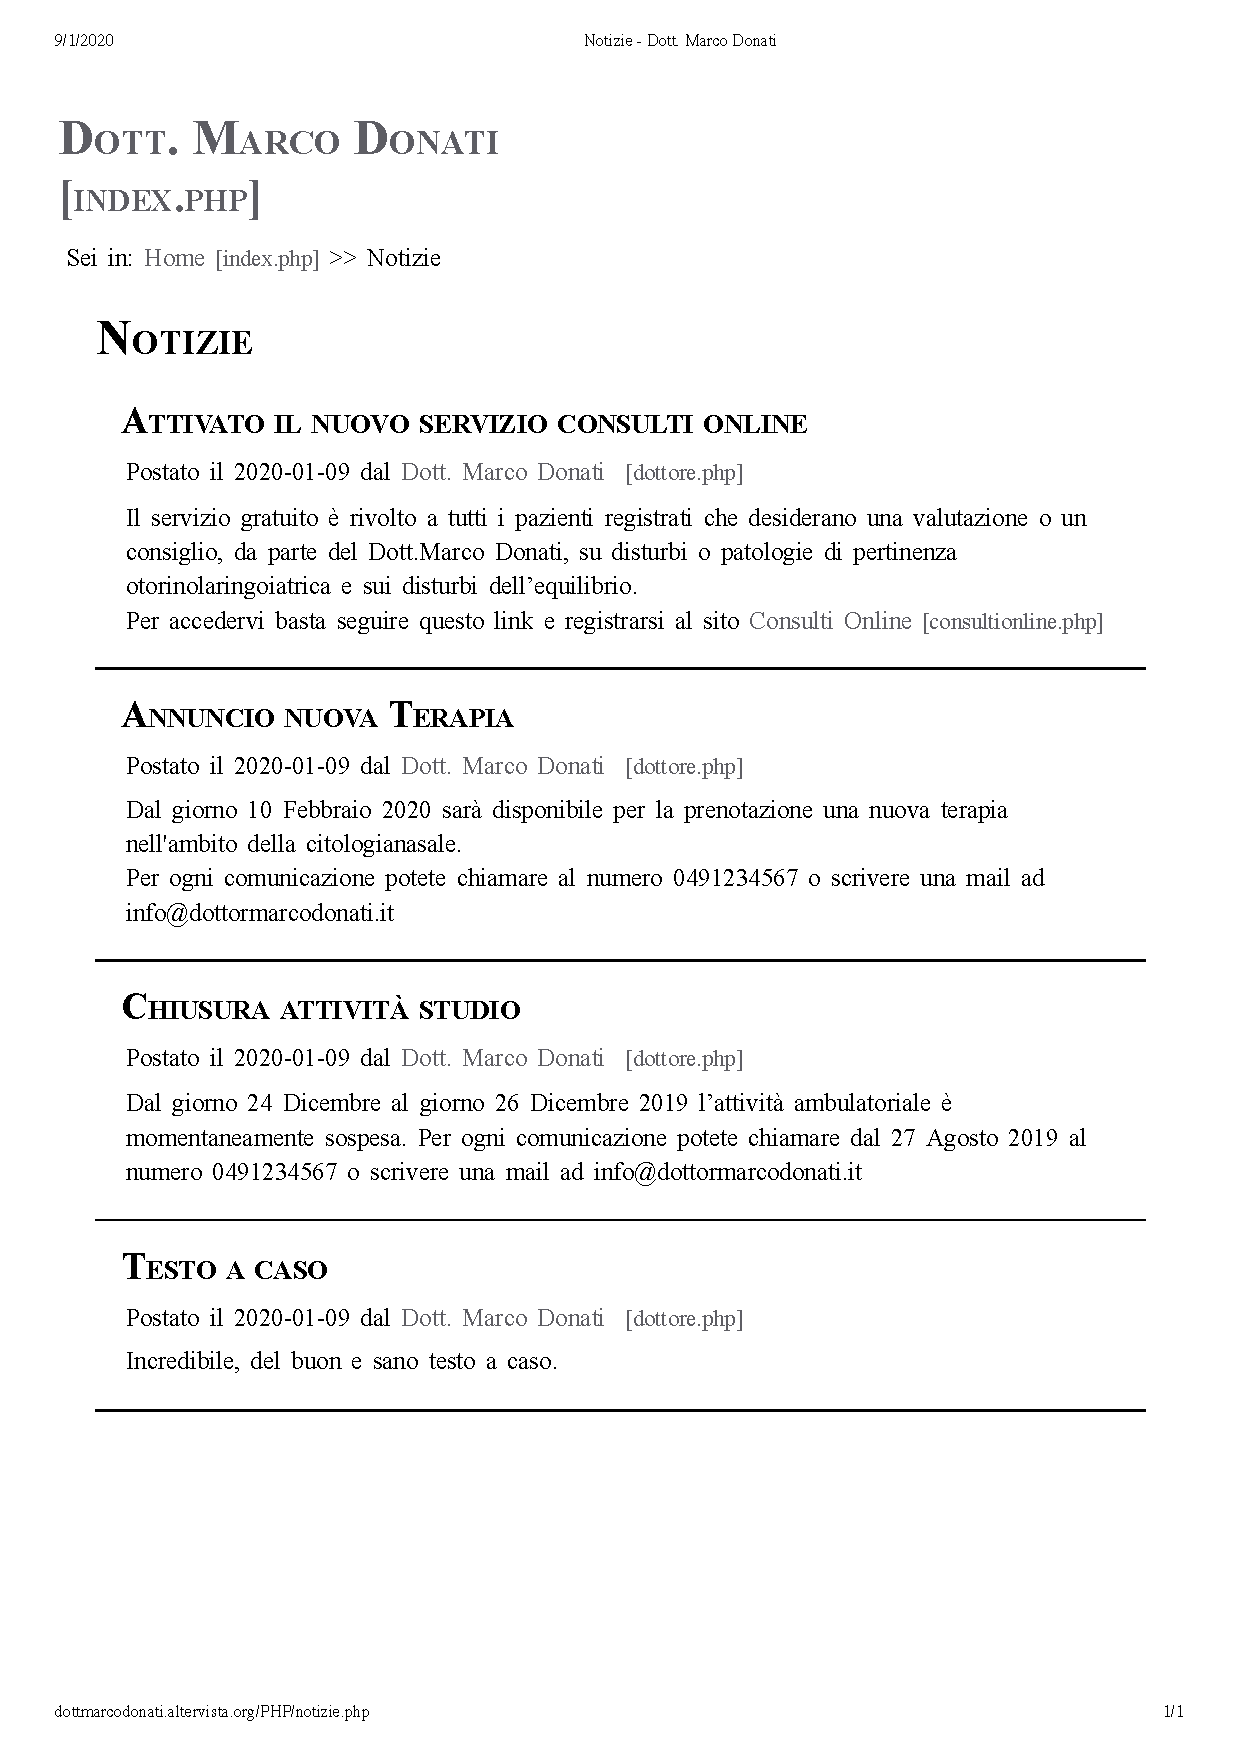
\includegraphics[width=12cm]{../img/stampa.pdf}
\end{center}
\captionof{figure}{Esempio di una pagina di stampa, in questo caso \textit{Notizie}}

\bigskip

\subsection{JavaScript}
Per il comportamento di alcune pagine del sito, lato client, è stato utilizzato uno script JavaScript, comprendente diverse funzioni. È stato scelto di limitare al massimo l’utilizzo di queste funzionalità, in quanto non è possibile fare nessuna assunzione sulla disponibilità di questa tecnologia. Il sito infatti rimane completamente navigabile e utilizzabile nel caso in cui JavaScript venga disabilitato o non sia comunque disponibile. Sono state quindi fornite tutte le alternative, lato server, attraverso PHP (unica alternativa in questo senso è rappresentata dallo slideshow, che degrada elegantemente mostrando solo una immagine statica).
Da mobile si presuppone ovvimante JavaScript attivo. \\

Le principali funzioni che abbiamo implementato (tutte contenute all’interno di un unico file) sono state:
\begin{itemize}
\item \textbf{validaAccedi()} : questa funzione controlla che tutti i campi immessi nel form specifico per l'accesso al sito siano corretti;
\item \textbf{validaRegistratii()} : questa funzione controlla che tutti i campi immessi nel form specifico per la registrazione al sito siano corretti;
\item \textbf{setPrenotaVisitaForJS()} : viene eseguita solo se c'è javascript;
questa funzione fa si che, per chi abbia JavaScript attivo, venga visualizzata la pagina come dovrebbe essere (con tutti i controlli e le chiamate alla pagina PHP per controllare la disponibilità), mentre per chi non dovesse avere JavaScript attivo, non venga eseguita questa funzione e quindi venga lasciata la pagina così com'è impostata in HTML, comunque utilizzabile;
\item \textbf{dataValida(date)} : funzione che controlla che la data sia inserita nel giusto formato (d/m/y);
\item \textbf{controllaDisponibilita()} : funzione che nasconde gli orari se non si riferiscono più al giorno selezionato, in caso di cambio data da parte dell'utente;
\item \textbf{openCloseMenu(menu)} : funzione per chiudere e aprire i menù a tendina nella versione mobile del sito;
\item \textbf{plusDivs(n)} : funzione per far scorrere lo slideshow;
\item \textbf{showDivs(n)} : funzione per mostrare le diverse immagini dello slideshow;
\item \textbf{changeFocusAccedi(event, campo)}: funzione che, al premere del tasto invio una volta che è stata inserita la email nel form per accedere al sito, passa il focus sul campo password, senza inviare direttamente il form. \\
\end{itemize}

\subsection{Compatibilità con browser datati}
Per garantire la compatibiltà con browser datati:
\begin{itemize}
\item All’interno dei form sono stati usati \textit{type text} per le email e il \textit{type number} per i numeri telefonici, scegliendo quindi di non utilizzare \textit{type email} e \textit{type tel};
\item \textit{sticky} viene messa in coda al codice come tutte le altre funzioni CSS3,  così che, se la pagina venisse aperta da un browser che non supporta CSS3 la funzionalità della pagina non verrebbe compromessa; semplicemente le funzioni CSS3 opzionali non sarebbero mostrate. Questo vale anche per proprietà come \textit{border-radius}, \textit{box-sizing};
\item Non usando CSS3 non è possibile fare radio button colorati, quindi un user di IE8 o precedenti vedrà solo dei pallini senza colore. Questo però non inficerà sulla usabilità perché i radio button cliccabili saranno comunque distinguibili da quelli non cliccabili;
\item Come detto in precedenza in §\ref{frontend:css} abbiamo usato \textit{@media flex}, questa proprietà CSS3, pur non essendo supportata dai vecchi browser, non degrada in modo particolare il sito. Anzi è solo una questione puramente estetica;
\item Per quanto riguarda la mappa di Google Maps, per utilizzarne la funzionalità non abbiamo avuto scelta se non usare funzioni HTML 5, che quindi risultano errate in un validatore xHTML 1.0 Strict. (Come è stato detto a lezione);
Quindi nella pagina contatti, il documento è stato dichiarato come HTML 5, unica eccezione del nostro sito.
\end{itemize}

